% This bring summarise and bring together all the previous section into a specification that should be fully expanded in the appendix with the following points, in providing what is known as the System Requirements Specification (SRS). This collects various information that you have previously agreed and worked on such as the UML diagrams.

\section{Purpose}

\section{Scope}

\section{System Overview}

\section{References}

\section{Definitions}

\section{Use Cases}
\begin{figure}[H]
    \centering
    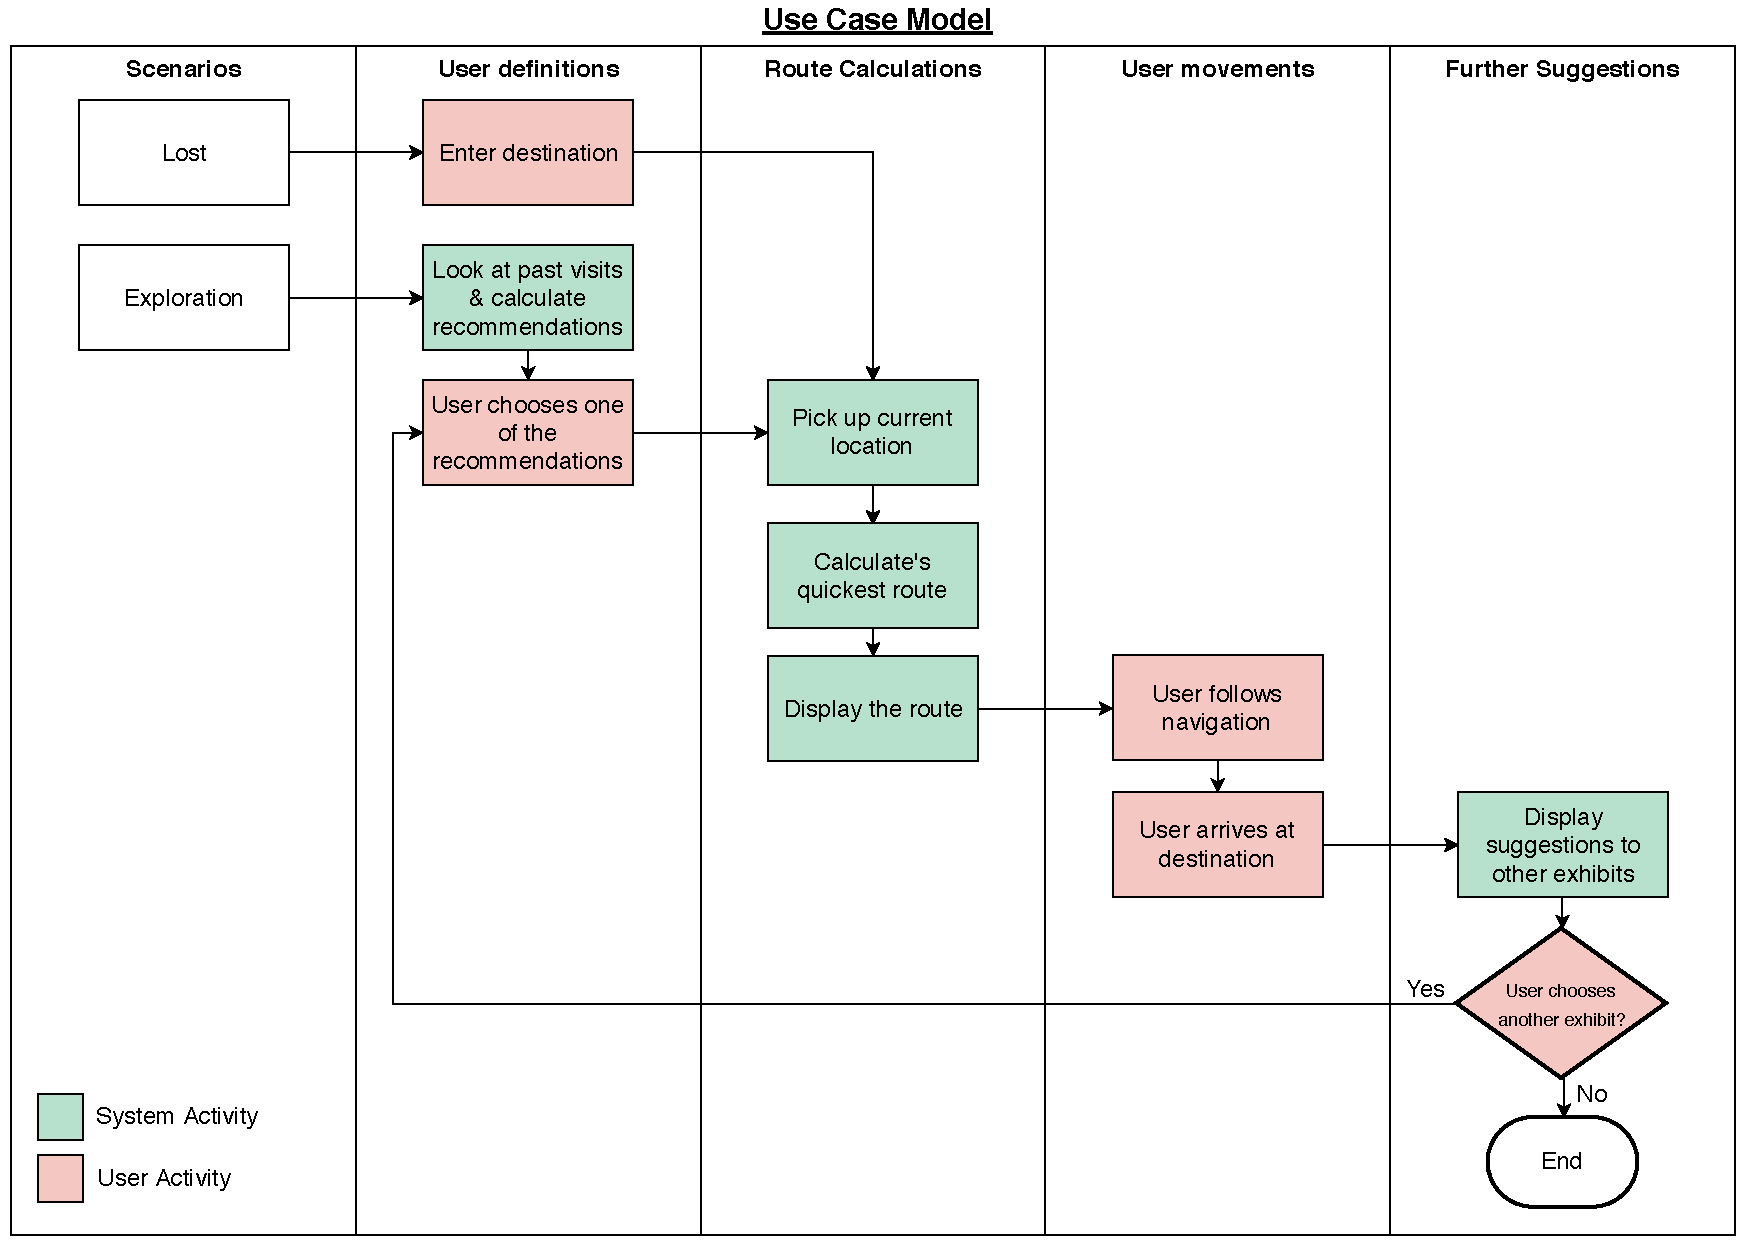
\includegraphics[width=\textwidth]
    {assets/use_case.pdf}
    \caption{Use Case Diagram}
    \label{fig:Use Case Diagram}
\end{figure}

\begin{figure}[H]
    \centering
    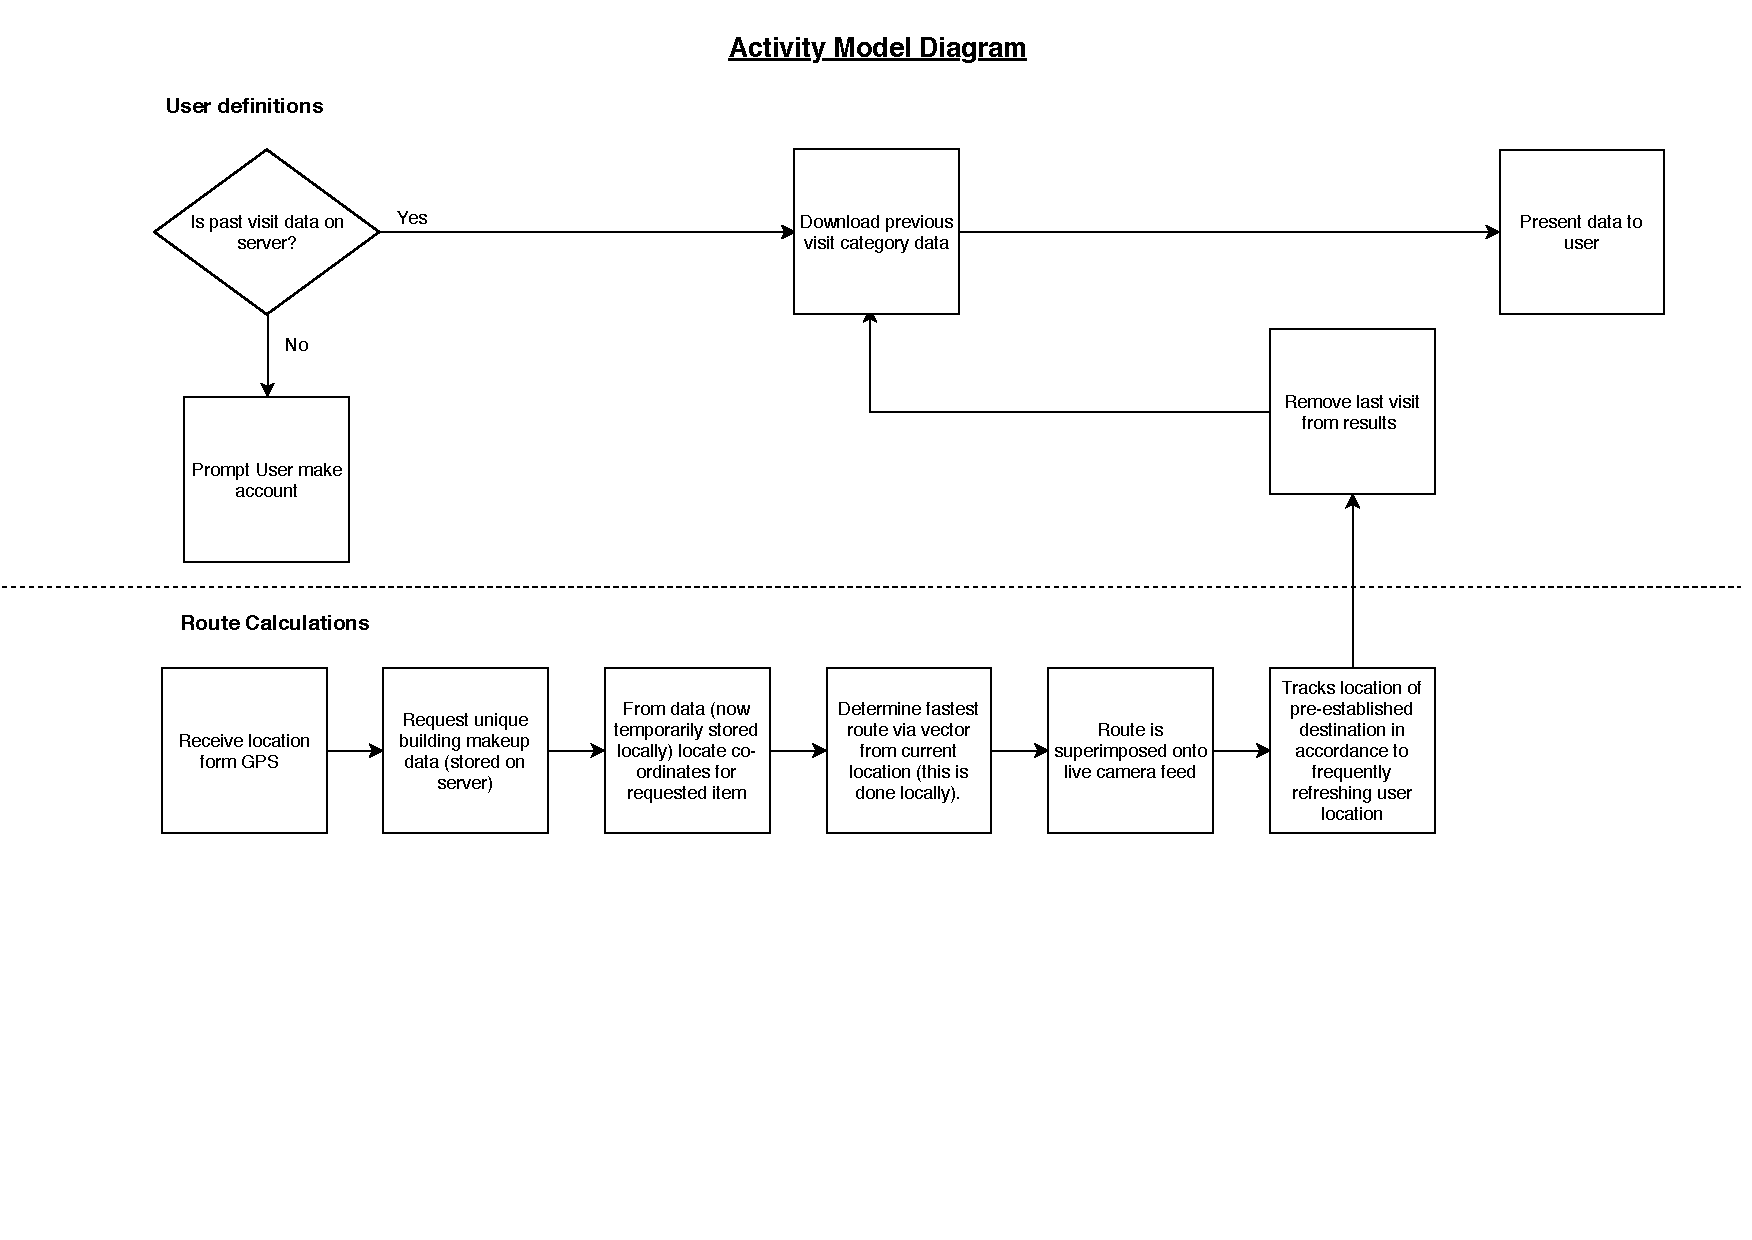
\includegraphics[angle=90, width=\textwidth]
    {assets/Activity_Diagram.pdf}
    \caption{Activity Model Diagram}
    \label{fig:Activity Model Diagram}
\end{figure}

\begin{figure}[H]
    \centering
    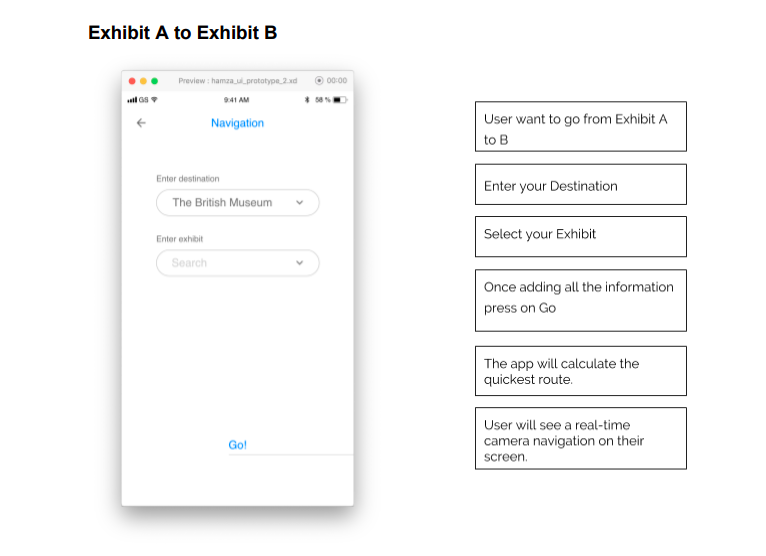
\includegraphics[width=\textwidth]
    {userstory_aTob.png}
    \caption{Going from point A to point B}
    \label{fig:AtoB}
\end{figure}

\begin{figure}[H]
    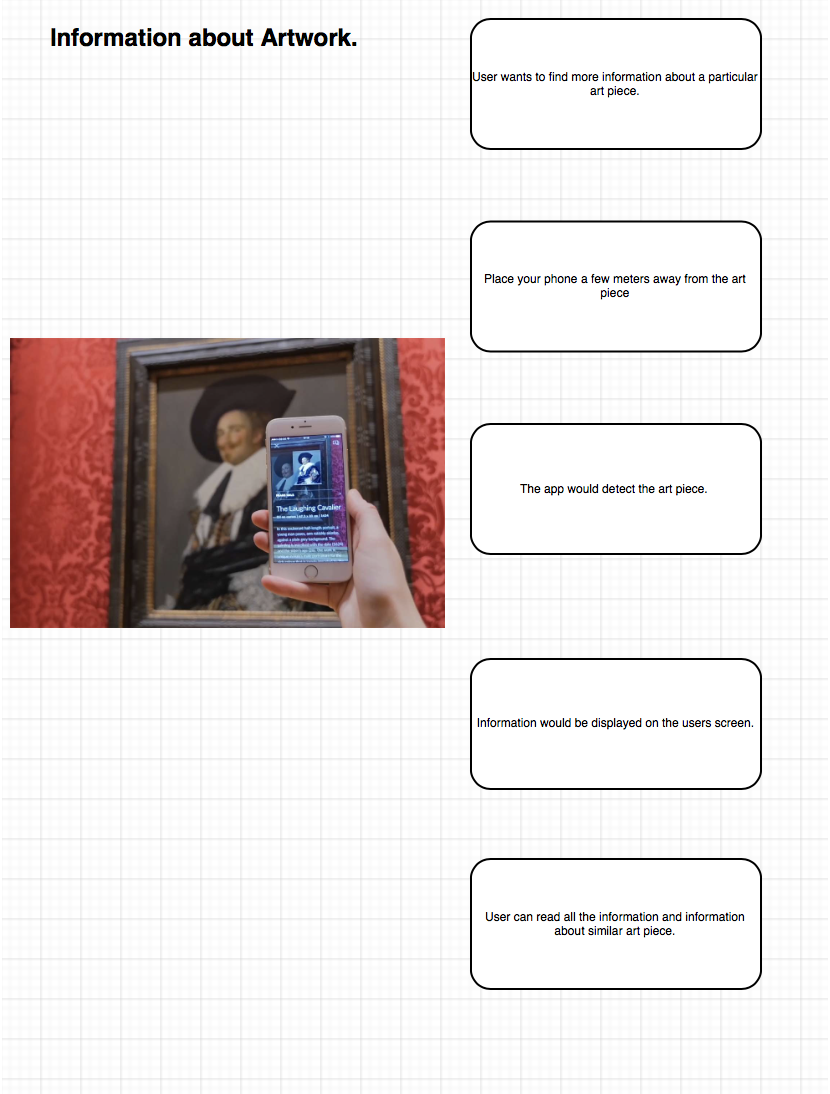
\includegraphics[width=\textwidth]
    {userstory_info.png}
    \caption{Getting information from exhibition}
    \label{fig:infofromexhibit}
\end{figure}

\begin{figure}[H]
    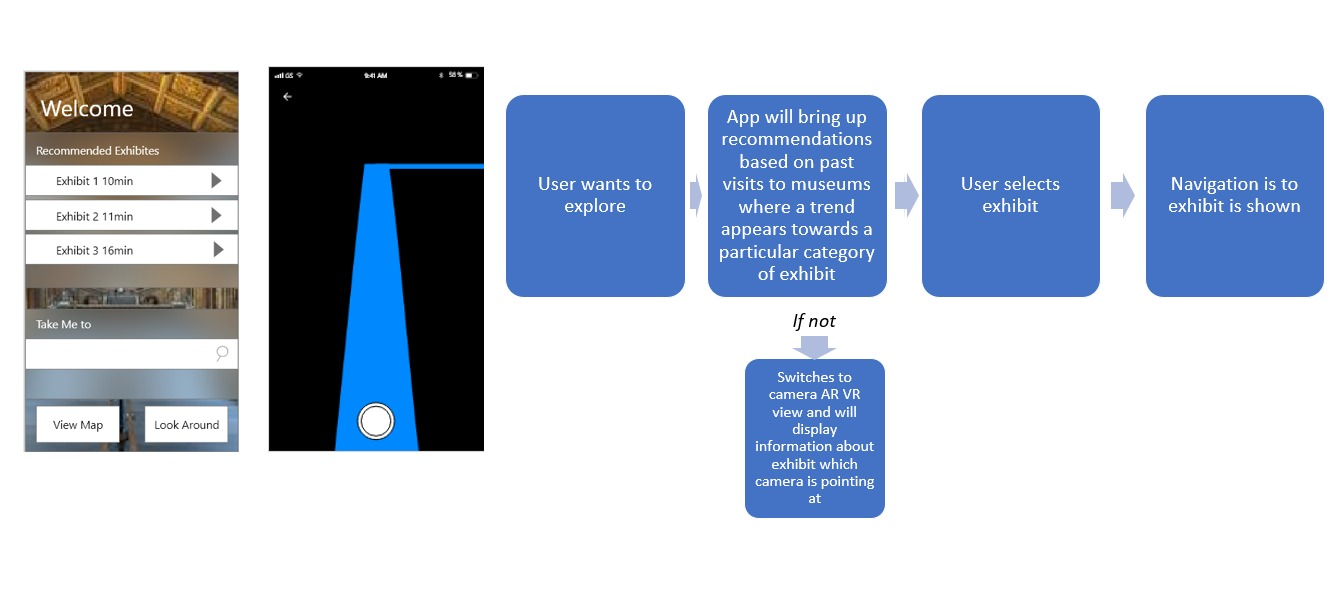
\includegraphics[width=\textwidth]
    {userstory_explore.jpeg}
    \caption{Exploring the museum}
    \label{fig:exploring}
\end{figure}

\section{Functional requirements}

\section{Non-functional requirements}